\documentclass[conference]{IEEEtran}
\IEEEoverridecommandlockouts
% The preceding line is only needed to identify funding in the first footnote. If that is unneeded, please comment it out.
\usepackage{cite}
\usepackage{amsmath,amssymb,amsfonts}
\usepackage{algorithmic}
\usepackage{graphicx}
\usepackage{textcomp}
\usepackage{xcolor}
\usepackage{enumitem} 
\usepackage{float}
\def\BibTeX{{\rm B\kern-.05em{\sc i\kern-.025em b}\kern-.08em
    T\kern-.1667em\lower.7ex\hbox{E}\kern-.125emX}}
\begin{document}

\title{Medical Abstract Segmentation}

\author{\IEEEauthorblockN{Saifuddin Shaikh}
\IEEEauthorblockA{\textit{Department of Information Technology} \\
\textit{Pune Institute of Computer Technology}\\
Pune, India \\
emmanuelm@pict.edu}
\and 



\IEEEauthorblockN{Dr. Emmanuel M.}
\IEEEauthorblockA{\textit{Department of Information Technology} \\
\textit{Pune Institute of Computer Technology}\\
Pune, India \\
saifuddinshaikh818@gmail.com} \\

\IEEEauthorblockN{Rishikesh Suryavanshi}
\IEEEauthorblockA{\textit{Department of Information Technology} \\
\textit{Pune Institute of Computer Technology}\\
Pune, India \\
rishits321@gmail.com}

\and


\IEEEauthorblockN{Pranish Warke}
\IEEEauthorblockA{\textit{Department of Information Technology} \\
\textit{Pune Institute of Computer Technology}\\
Pune, India \\
pranish2402@gmail.com}




}

\maketitle

\begin{abstract}
Randomized control trials (RCTs) are essential for evaluating the effectiveness of medical interventions, but their results are often buried within lengthy and complex documents. Efficiently extracting and organizing critical information from RCT abstracts can significantly impact evidence-based decision-making and healthcare research.
The automated segmentation of medical abstracts is a vital component of medical information retrieval and analysis, significantly impacting clinical decision-making, healthcare research, and knowledge discovery. 
 This paper presents an innovative approach to segmenting abstracts of RCTs through the application of natural language processing (NLP) and neural networks.
 The practical applications of NLP and neural network-based text segmentation in the context of RCTs are exemplified, ranging from systematic reviews and meta-analyses to the development of clinical guidelines. Case studies are presented to showcase the impact of this technology in improving the accessibility and utilization of RCT results.
This paper serves as a valuable resource for researchers, healthcare professionals, and data scientists, offering a glimpse into the future of RCT abstract segmentation. It underscores the pivotal role of NLP and neural networks in unlocking the potential of RCT data, ultimately advancing the field of evidence-based medicine and healthcare decision-making.



\end{abstract}

\begin{IEEEkeywords}
medical abstract,text segmentation,randomized control trial (RCT),natural language processing(NLP),neural networks.
\end{IEEEkeywords}

\section{Introduction}
Randomized Controlled Trial (RCT) is a specific type of study design commonly used in medical research to evaluate the effectiveness of a treatment or intervention. In an RCT, participants are randomly assigned to different groups to compare the outcomes of those who receive the treatment or intervention with those who do not.  Existing models based on artificial neural networks (ANNs) for sentence classification often do not incorporate the context in which sentences appear and classify sentences individually.

The scope of medical abstract segmentation for RCTs using NLP and neural networks encompasses a wide range of applications that contribute to the advancement of healthcare, medical research, and clinical decision-making. This field continues to evolve, driven by the increasing volume of medical literature and the need for more efficient ways to extract valuable insights from this vast body of knowledge.

For a variety of Natural Language Processing (NLP) activities, such as information retrieval, information extraction, and text summarization, structuring the unstructured Randomized Controlled Trial (RCT) is helpful. One example is classifying sentences into Background, Objective, Methods, Results, and Conclusion. However, a large number of PubMed abstracts lack hierarchical organization. Only about 30\% of all PubMed abstracts, according to Ripple et al. (2014), include their structural information, which hinders effective knowledge discovery and information retrieval from those sizable biomedical bibliographic databases. Sentence classification for medical abstracts has been the subject of a lot of studies. 

The aim of "Medical Abstract Segmentation" is to focus on classifying sentences in medical abstracts, and particularly in randomized controlled trials (RCTs), as they are commonly considered to be the best source of medical evidence.

 


\section{Literature Survey}

A comprehensive study has been done on text classification in the domain of medical research papers. Some of the most recent and prominent ones have been used for this literature survey. 

In [1] the dataset consists of approximately 200,000 abstracts of randomized controlled trials, totaling 2.3 million sentences. Each sentence of each abstract is labeled with its role in the abstract using one of the following classes: background, objective, method, result, or conclusion, and PubMed 200k RCT is a substantial dataset designed for sequential sentence classification, is introduced. It notably stands as one of the largest datasets of its kind known to date. The evaluation encompasses the performance assessment of various baseline models, providing a valuable reference for researchers to readily benchmark their algorithms without the necessity of creating their own foundational benchmarks.

[2] suggests a novel uniform deep learning architecture and multi-task learning approach for cross-domain sequential sentence classification in scientific texts. This paper introduces a comprehensive deep-learning architecture designed for sequential sentence classification, demonstrating remarkable advancements, particularly in full paper datasets, without the need for intricate feature engineering. The authors conduct a thorough investigation and comparison of transfer learning approaches, shedding light on the exceptional effectiveness of multi-task models applied across diverse datasets. Furthermore, this study places significant emphasis on the crucial notion of semantic relatedness between classes within varying dataset annotation schemes. It proposes a practical and robust method for identifying and establishing these semantic connections. Such an approach bears the promise of unlocking the potential for cross-discipline applications in the domain of sentence classification, with particular relevance to academic search engines and information retrieval systems.

Similarly [3] Adopted a deep learning neural network model and pretrained the network on PubMed non-RCT dataset. Transfer Learning with fine-tuning was done on the hand-labeled dataset they created from scratch. The PubMed-non-RCT corpus was converted into a three-class dataset, and their model was trained on it. They achieved 92.1\% accuracy on the PubMed-non-RCT dataset. The model was then evaluated on various CS corpora using different approaches: 'Locally-trained,' 'Pre-trained on PubMed,' and 'Fine-tuned'. Notably, 'Fine-tuned' transfer learning significantly improved the model, while 'Pre-trained on PubMed' performed worse than local training, indicating the dissimilarity between the CS and biomedical corpora. Despite such differences, transfer learning with fine-tuning still provided more than a 10\% accuracy boost, even with entirely dissimilar datasets. The paper introduces a method for automatic discourse classification in computer science abstracts, showing that transfer learning with fine-tuning yields impressive results, even with limited labeled data. The model effectively generalizes across CS sub-fields, despite variations in discourse classification due to presentation style differences.

In [4] The model is composed of four components: the word embedding layer, the sentence encoding layer, the context enriching layer, and the label sequence optimization layer. The sequence of embedding vectors is first processed by a bi-directional RNN (bi-RNN) or CNN layer. In this work, they introduced an ANN-based hierarchical sequential labeling network designed to classify sequentially appearing sentences in text. By incorporating contextual information from neighboring sentences through an LSTM layer, they observed a significant enhancement in prediction quality. Their model demonstrated a notable 2\%-3\% improvement over state-of-the-art results in two datasets focusing on sequential sentence classification within medical abstracts. This proposed model's potential for generalization to various problems related to sequential sentence classification, including paragraph-level sequential sentence categorization in full-text articles, presents promising opportunities for text mining and document retrieval.

In [5] The model consists of two novel components: supervised local attention and an auxiliary span-based classification task. The proposed model aims to capture the latent segment structure of the document by considering the coherent semantics of contiguous sentences. It utilizes dynamic local attention to explicitly capture the structural information. 

In [6] a Machine Learning approach that aims to classify sentences according to the PIBOSO scheme is presented. A discriminative set of features that do not rely on any external resources to achieve results is used. In this paper, they introduced a machine-learning approach for identifying scientific artifacts in biomedical abstracts within the context of Evidence-Based Medicine. Their approach utilized sentence classification following the PIBOSO scheme. Importantly, their approach did not rely on external resources for classification features. The results demonstrated a significant improvement over existing methods, achieving a micro-average F-score of 90.74\% and 87.21\% for structured and unstructured abstracts, respectively. This marks a substantial increase compared to prior approaches.

In [7] visits clustering algorithm is implemented based on the following four steps:  Medical concepts are extracted from free-text descriptions of an interview and examination, a new representation of identified concepts is derived using concept embedding, concept embeddings are transformed into visit embeddings and clustering is performed on visit embeddings. They used two of the most common: k-means and hierarchical clustering with Ward’s method for merging clusters.  These algorithms cover two different clustering approaches. The algorithms are memory and time-efficient, so no need to use more advanced methods. 

[8] and [9] propose a few-shot prompt learning-based approach to classify sentences in medical abstracts of randomized clinical trials (RCT) and observational studies (OS) to subsections of Introduction, Background, Methods, Results, and Conclusion. 5 manually designed templates in a combination of 4 BERT model variants were tested and compared to a previous Hierarchical Sequential Labeling Network architecture and traditional BERT-based sentence classification method. Four deep learning models, namely RNN, LSTM, GRU, and BLSTM are used. Data pre-processing steps are applied that include: text cleaning, tokenization, stemming, as well as lemmatization to remove and stop words. Their approach achieves state-of-the-art results on all three datasets, surpassing Jin and Szolovits (2018) and their BERT-based baselines. The performance gap between their baselines and their best model is more pronounced for smaller datasets (CSABSTRUCT, NICTA) and narrower for the larger dataset (PUBMED-RCT), underlining the significance of pretraining for smaller datasets. To delve into the advantages of their joint sentence encoding relative to the BERT+Transformer baseline, they qualitatively analyze examples from CSABSTRUCT. They discover that a significant portion of such examples require contextual information for accurate classification, emphasizing the need for context in certain instances.


\begin{table*}%[h]
\begin{tabular}{|p{4.6cm}|p{6cm}|p{4.9cm}|p{1.95cm}|}
\hline
Title &
  Methodologies &
  Inferences &
  Dataset \\ \hline
\begin{tabular}[c]{@{}l@{}}PubMed 200k RCT: a Dataset for \\ Sequential Sentence \\ Classification in Medical Abstracts\end{tabular} &
  \begin{tabular}[c]{@{}l@{}}Dataset is constructed upon MED-\\ LINE/PubMed Baseline Database. \\ Abstracts are selected based on the\\ two criteria: \\ i. It must be an RCT\\ ii. It must be structured\end{tabular} &
  \begin{tabular}[c]{@{}l@{}}• It is the largest such dataset \\    in the field of Medical \\    Research.\\ • It evaluated the performance on \\   several baseline models \\   based on this dataset.\\ • It achieved state of the art results \\   for Bi-ANN model with \\   F1 score of 91.6\end{tabular} &
  \begin{tabular}[c]{@{}l@{}}PubMed \\ 200k RCT\end{tabular} \\ \hline
\begin{tabular}[c]{@{}l@{}}Cross-Domain Multi-Task \\ Learning for Sequential Sentence \\ Classification in Research Papers\end{tabular} &
  \begin{tabular}[c]{@{}l@{}}1. Proposed SciBERT-HSLN architecture.\\ 2. Utilized SciBERT for Word Embeddings.\\ 3. Two approaches are suggested here one \\ without Transfer Learning and one with \\     Transfer Learning.\end{tabular} &
  \begin{tabular}[c]{@{}l@{}}• It achieved state of the art results for \\    PMD dataset with F1 score of 93.1\\ • F1 score of 86.8 for NIC dataset\end{tabular} &
  \begin{tabular}[c]{@{}l@{}}PMD, NIC, \\ ART, DRI\end{tabular} \\ \hline
\begin{tabular}[c]{@{}l@{}}Segmenting Scientific Abstracts \\ into Discourse Categories: \\ A Deep Learning-Based Approach \\ for Sparse Labeled Data\end{tabular} &
  \begin{tabular}[c]{@{}l@{}} Transfer Learning with Fine Tuning was \\ done on the hand labelled dataset \\ they created from scratch.\end{tabular} &
  \begin{tabular}[c]{@{}l@{}}• It was able to achieve 75\% accuracy \\    with the classification of CS abstracts.\end{tabular} &
  \begin{tabular}[c]{@{}l@{}}Hand Labelled \\ corpus of \\ structured \\ CS abstracts\end{tabular} \\ \hline
\begin{tabular}[c]{@{}l@{}}Hierarchical Neural Networks \\ for Sequential Sentence \\ Classification in Medical \\ Scientific Abstracts\end{tabular} &
  \begin{tabular}[c]{@{}l@{}} Model is composed of four layers :\\     i.   Word Embedding layer\\     ii.  Sentence Encoding layer\\     iii. Context Enriching layer\\     iv.  Label Sequence Optimisation layer\end{tabular} &
  • F1 score for PubMed 20k dataset is 92.6 &
  PubMed 20k RCT \\ \hline
\begin{tabular}[c]{@{}l@{}}A Span-based Dynamic\\  Local Attention Model for \\ Sequential Sentence \\ Classification\end{tabular} &
  \begin{tabular}[c]{@{}l@{}} Model consists of two novel components:\\       i. supervised local attention\\       ii. auxiliary span based classification\end{tabular} &
  \begin{tabular}[c]{@{}l@{}}• F1 score of 92.8 on PubMed 20k RCT \\ • F1 score of 86.8 on NICTA-PIBOSO\end{tabular} &
  PubMed 20k RCT \\ \hline
\begin{tabular}[c]{@{}l@{}}Identifying scientific artefacts \\ in biomedical literature: \\ the Evidence Based Medicine \\ use case\end{tabular} &
  \begin{tabular}[c]{@{}l@{}}A machine learning approach that aims \\     to classify sentences according to\\     PIBOSO scheme is presented.\end{tabular} &
  \begin{tabular}[c]{@{}l@{}}• CRF classifier achieves F1 score of 90.74 \\    and 87.21 respectively over structured \\    and unstructured abstracts.\end{tabular} &
  NICTA-PIBOSO \\ \hline
\begin{tabular}[c]{@{}l@{}}Towards More Generalizable and \\ Accurate Sentence \\ Classification in \\ Medical Abstracts with Less Data\end{tabular} &
  \begin{tabular}[c]{@{}l@{}} Few shot prompt based learning approach to \\     classify\\     sentences in medical abstracts was discussed.\end{tabular} &
  \begin{tabular}[c]{@{}l@{}}• The study showed that the HSLN model \\    required only 20\% of the training data to \\    achieve comparable F1 scores when \\    compared with the baseline model.\end{tabular} &
  \begin{tabular}[c]{@{}l@{}}PubMed 200k/20k\\ PubMed 20k OS\end{tabular} \\ \hline
\begin{tabular}[c]{@{}l@{}}Interpretable segmentation \\ of medical free-text records \\ based on word\end{tabular} &
  \begin{tabular}[c]{@{}l@{}} K-Means and Hierarchical Clustering with \\ Ward's method was used.\end{tabular} &
  \begin{tabular}[c]{@{}l@{}}• The embeddings outperformed \\    Pennington \\    et al on medical term analogies despite a \\    smaller corpus size.\\ • Future work should explore the dynamic \\    relationship with identified clusters.\end{tabular} &
  \begin{tabular}[c]{@{}l@{}}The Polish corpus \\ of free text \\ clinical records\end{tabular} \\ \hline
\begin{tabular}[c]{@{}l@{}}Pretrained Language Models\\  for Sequential Sentence\\ Classification\end{tabular} &
  \begin{tabular}[c]{@{}l@{}} Four Deep Learning Models namely RNN, LSTM,\\     GRU and BLSTM are used.\end{tabular} &
  \begin{tabular}[c]{@{}l@{}}• Accuracy: BLSTM gives the highest \\    accuracy of 82.18\%\end{tabular} &
  \begin{tabular}[c]{@{}l@{}}Kaggle Dataset \\ having insult \\ labelled \\ comments \\ was used.\end{tabular} \\ \hline
\begin{tabular}[c]{@{}l@{}}Deep Learning Based Text Classification: \\ A Comprehensive Review\end{tabular} &
  \begin{tabular}[c]{@{}l@{}} Survey of more than 150 DL models was carried, \\     which are developed in the past six years \\     and have significantly improved \\     state of the art on various TC tasks\end{tabular} &
  \begin{tabular}[c]{@{}l@{}}• Several state of the art models were used\\    in this paper\end{tabular} &
  \begin{tabular}[c]{@{}l@{}}SQuAD,\\ WikiQA,\\ DBpedia\end{tabular} \\ \hline
\begin{tabular}[c]{@{}l@{}}Universal Language Model Fine-\\ tuning for Text Classification.\end{tabular} &
  \begin{tabular}[c]{@{}l@{}}\\  Proposed discriminative fine-tuning, slanted \\     triangular learning rates, and gradual unfreezing\end{tabular} &
  \begin{tabular}[c]{@{}l@{}}• Method suggested significantly \\    outperforms \\    the state-of-the-art  on six text \\    classification tasks, reducing the error  \\    by 18-24\% on the majority \\    of datasets.\end{tabular} &
  \begin{tabular}[c]{@{}l@{}}TREC-6\\ IMDb\\ Yelp-bi Yelp-full\\ DBpedia\\ AG\end{tabular} \\ \hline
\begin{tabular}[c]{@{}l@{}}A Hierarchical Model with Recurrent \\ Convolutional \\ Neural Networks for \\ Sequential Sentence Classification\end{tabular} &
  \begin{tabular}[c]{@{}l@{}} A new approach called SR-RCNN to generate \\     sentence encoding which uses both Bi-RNN \\     and text CNN to capture contextual and literal \\     relevance information\end{tabular} &
  \begin{tabular}[c]{@{}l@{}}• The model performs best on all datasets, \\    promoting previous best published \\    results by 0.5\%, 0.5\%and 2.5\% \\    on the PubMed 20k, PubMed 200k \\    and NICTA-PIBOSO dataset\end{tabular} &
  \begin{tabular}[c]{@{}l@{}}PubMed RCT,\\ NICTA-PIBOSO\end{tabular} \\ \hline
\begin{tabular}[c]{@{}l@{}}Sectioning of Biomedical Abstracts: \\ A Sequence of Sequence\\ Classification Task.\end{tabular} &
  \begin{tabular}[c]{@{}l@{}}1. It uses BIOBERT based model, with a moving\\     window to contextualise the abstracts.\\ 2. Proposed SSN-4 Model which has four layers:\\          i. word embedding layer\\          ii. sentence representation layer\\          iii. BLSTM layer\\          iv. CRF layer\end{tabular} &
  \begin{tabular}[c]{@{}l@{}}• The model trained with the MDS \\    performs fairly well in \\    both MDS and RCT data sets\end{tabular} &
  \begin{tabular}[c]{@{}l@{}}A new data set \\ called MDS \\ that is \\ considerably \\ bigger than \\ PubMed RCT\end{tabular} \\ \hline
\end{tabular}
\end{table*}



\section{Methodology}
\begin{figure}[H]
    \centering
    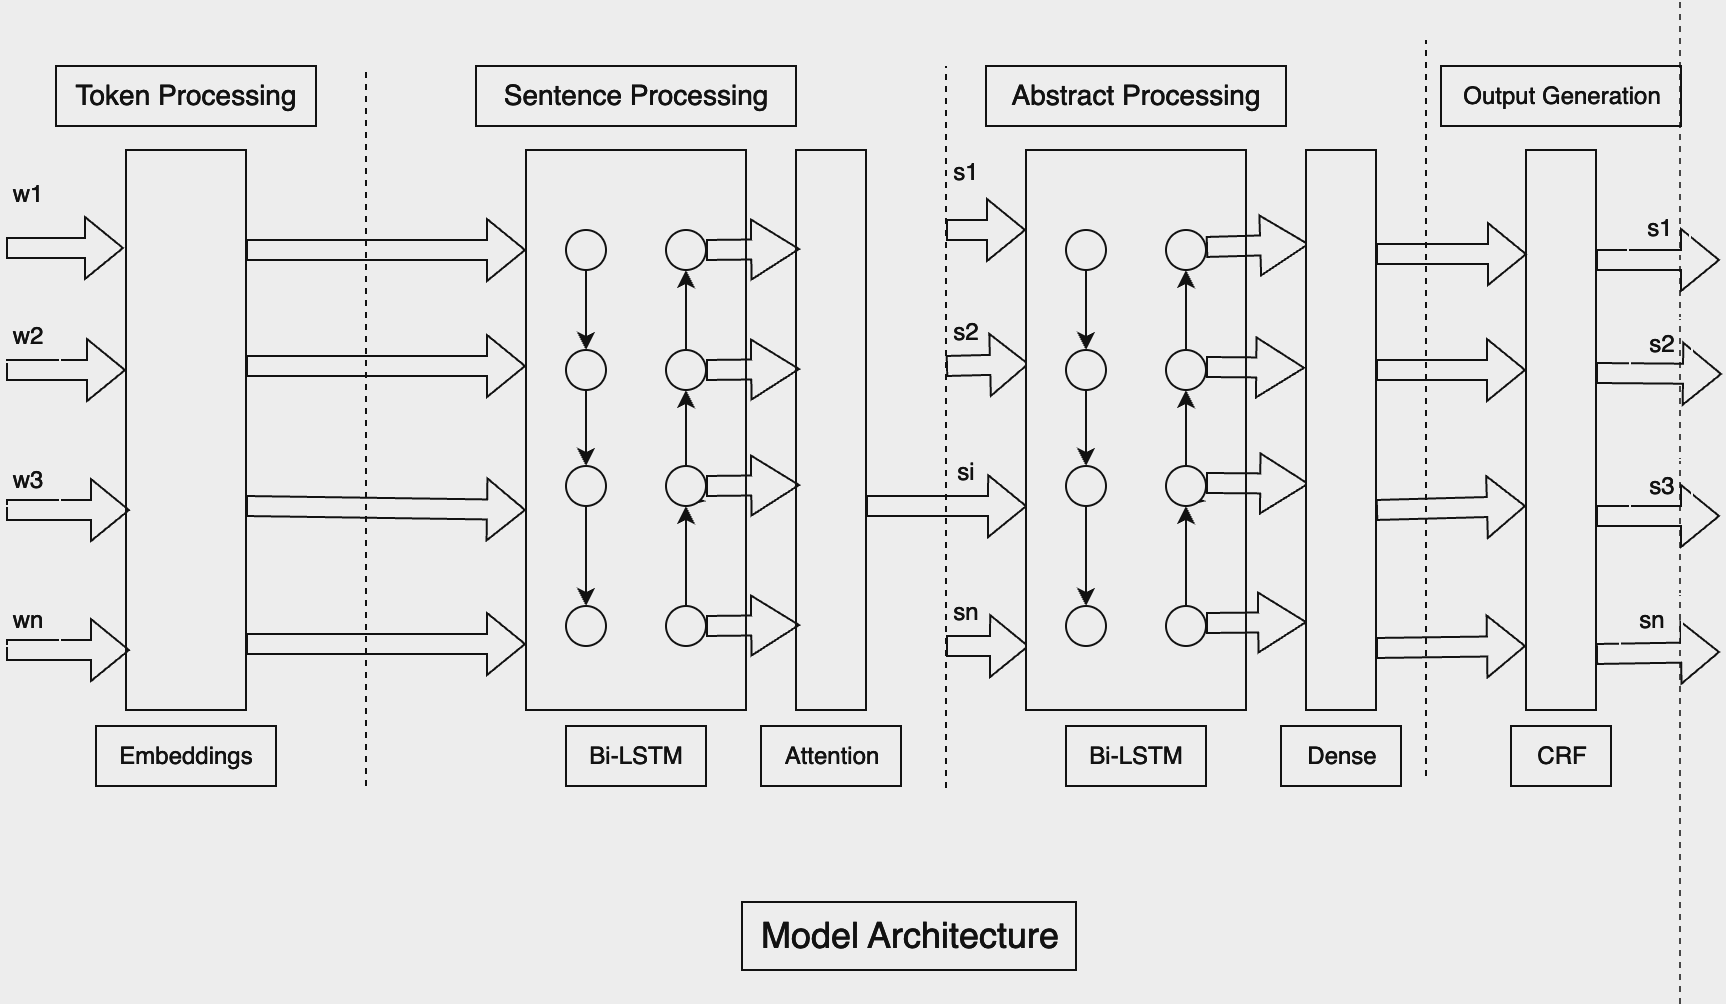
\includegraphics[width=8cm]{model_architecture.png}
    \caption{Model Architecture}
    \label{fig:architecture}
\end{figure}

The Hierarchical Sequential Labeling Network (HSLN) serves as the foundation for our method, which we refer to as PubMedBERT-HSLN. We assess the method on RCT abstracts using PubMedBERT as word embeddings.This research aims to present an empirical investigation on transfer learning and propose a uniform solution, rather than to surpass state-of-the-art results. The levels of our PubMedBERT-HSLN architecture are as follows:
 \begin{enumerate}[label=\Roman*., itemsep=10pt]
    \item Word Embeddings:
          A series of tokens (t1,t2,...,tm) from the phrase si is the input, while a sequence of (PubMedBERT) word embeddings (s1,s2,...,sm) is the output.
    \item Sentence Encoding:
          A Bi-LSTM is used to convert the input (w1,w2,...,wm) into representations (h1,h2,...,hm) that are enhanced with contextual information from the phrase.
    \item Context Enrichment:
          Sentence vectors (e1,e2,...,en) are converted into (c1,c2,...,cn) using a Bi-LSTM.As a result, context from adjacent sentences enriches each sentence vector ci.
    \item Output Layer:
          A CRF layer predicts the labels which acts like a final output layer based on highest conditional joint probability.
    
\end{enumerate}
\subsection{Dataset}
The PubMed 20K RCT dataset was used in this study. The dataset is available at https://github.com/Franck- Dernoncourt/pubmed-rct.
The collection includes 2.3 million phrases from almost 200,000 abstracts of randomized controlled trials. Each abstract's sentences are assigned a class based on their role in the abstract, such as background, objective, method, result, or conclusion.


For the specified problem of medical abstract segmentation, PubMed dataset is publicly available. It consists of following five labels and the number of samples are as follows:

1. METHODS          59353

2. RESULTS          57953

3. CONCLUSIONS      27168

4. BACKGROUND       21727

5. OBJECTIVE        13839

\subsection{Types of classification}

Sentence classification is a common task in natural language processing (NLP) and can be categorized into various types, depending on the specific problem or goal. Here are some common types of sentence classification:

1.Text Classification : 
    \begin{itemize}
        \addtolength{\leftmargin}{10pt}
        \item Sentiment Analysis
        \item Sequential Sentence Classification
        \item Topic Classification
    \end{itemize}

2.Language Understanding:
    \begin{itemize}
        \addtolength{\leftmargin}{10pt}
        \item Named Entity Recognition
        \item Part-of-Speech (POS) Tagging
    \end{itemize}
    
3.Document Summarization:
    \begin{itemize}
        \addtolength{\leftmargin}{10pt}
        \item Sentence Importance Ranking:
    \end{itemize}

4.Question Answering:
    \begin{itemize}
        \addtolength{\leftmargin}{10pt}
        \item Question Type Classification
        \item Answer Type Classification
    \end{itemize}


\subsection{Data import and cleaning}
The dataset was cloned from the publicly available github repository of [1]. The cloned PubMed RCT dataset consisted of four different sub-datasets within it.The four datasets are as follows :

1.PubMed\textunderscore200K\textunderscore RCT

2.PubMed\textunderscore200K\textunderscore RCT\textunderscore numbers\textunderscore replaced\textunderscore with\textunderscore at\textunderscore sign

3.PubMed\textunderscore20K\textunderscore RCT

4.PubMed\textunderscore20K\textunderscore RCT\textunderscore numbers\textunderscore replaced\textunderscore with\textunderscore at\textunderscore sign

Reading the lines from the training text file results in a list of strings containing different abstract samples, the sentences in a sample along with the role the sentence plays in the abstract.

The role of each sentence is prefixed at the start of each line separated by a tab (\textbackslash t) and each sentence finishes with a new line (\textbackslash n).

Different abstracts are separated by abstract ID's (lines beginning with \#\#\#) and newlines (\textbackslash n).

Prior to feature extraction, pre-processing is applied to the text to clean it and retain only the terms that provide valuable information for sentence classification. The cleaning function performs the following actions on the corpus:

1. Converting the text to lowercase.

2. Removal of Stopwords.

3. Stemming and Lemmatization. 

4. Tokenisation

After these steps, the dataset will be ready for feature engineering. 

\subsection{Feature Engineering}

The data should be transformed into a format that the
model can comprehend after being cleaned and preprocessed.
Feature engineering is a crucial step in the process of sequential sentence classification, a task commonly encountered in natural language processing (NLP) and text analysis. Sequential sentence classification involves assigning one or more labels to each sentence in a sequence, such as in sentiment analysis, named entity recognition, or text categorization. Effective feature engineering can significantly improve the performance of machine learning models used for this purpose.
There are various key aspects of Feature Engineering in Sequential Sentence Classification : 
\begin{enumerate}
    \item Text Representation
    \item Preprocessing
    \item Tokenization
    \item Feature Extraction
    \item Sequence Encoding
    \item Domain-Specific Knowledge
    \item Model Selection
\end{enumerate}

The major drawback of the two previous feature extraction techniques is the loss of the
relationship between words and, as a consequence, the context of a document. To overcome this problem,  a third extraction technique[10]
Word Embedding: The idea is to assign to similar terms close vectors of a continuous
and multidimensional vector space in a way that makes it possible to calculate similarities
between words or sentences thanks to the distance between vectors, as well as to
generalise a sentence into similar sentences, since the vectors will be similar[10].
Now another problem with this is about the context. If the same word is used for different context the word embedding fail to caputre this. 
This is overcomed by BERT which provides contextualized feature vectors.
We are planning to use the PubMedBERT which is a pretrained model on medical abstracts and literature.This model achieves state-of-the-art performance on several biomedical NLP tasks, as shown on the Biomedical Language Understanding and Reasoning Benchmark.      


\section{Conclusion and Future Scope}

Our work here contributes to the ongoing efforts for implementation of a Natural Language Processing (NLP) model designed for the segmentation of text lines in medical research paper abstracts.In this paper we extensively carried out empirical study of various deep learning models and explored particularly the bio-medical domain.The proposed model can be regarded as an initial benchmark, marking the starting point of an ongoing effort to construct an enhanced model.
For future enhancements, the following considerations merit attention:
Replacement of Universal Sentence Encoder (USE) with BiomedNLP-PubMedBERT-base-uncased-abstract : BiomedNLP-PubMedBERT-base-uncased-abstract presents a compelling alternative to USE in terms of performance and accuracy.

Text Preprocessing: The absence of text preprocessing in our proposed architecture was a deliberate choice, aimed at minimizing feature dependencies during model training, following a similar approach for the "current line" feature. Nevertheless, to further enhance model performance, it is recommended to consider text preprocessing techniques, such as the removal of stopwords, punctuation, special characters, and webpage links, conversion to lowercase, as well as the application of stemming and lemmatization. These strategies can contribute to more refined and accurate model predictions.

% \section*{Acknowledgment}

% The preferred spelling of the word ``acknowledgment'' in America is without 
% an ``e'' after the ``g''. Avoid the stilted expression ``one of us (R. B. 
% G.) thanks $\ldots$''. Instead, try ``R. B. G. thanks$\ldots$''. Put sponsor 
% acknowledgments in the unnumbered footnote on the first page.

% \section*{References}
% \cite{b1}V. Kumar, S. Pasari, V. P. Patil and S. Seniaray, "Machine Learning based Language Modelling of Code Switched Data," 2020 International Conference on Electronics and Sustainable Communication Systems (ICESC), Coimbatore, India, 2020, pp. 552-557, doi: 10.1109/ICESC48915.2020.9155695.
% \cite{b2}Rahul, H. Kajla, J. Hooda and G. Saini, "Classification of Online Toxic Comments Using Machine Learning Algorithms," 2020 4th International Conference on Intelligent Computing and Control Systems (ICICCS), Madurai, India, 2020, pp. 1119-1123, doi: 10.1109/ICICCS48265.2020.9120939. 
% \cite{b3}T. Tang, X. Tang and T. Yuan, "Fine-Tuning BERT for Multi-Label Sentiment Analysis in Unbalanced Code-Switching Text," in IEEE Access, vol. 8, pp. 193248-193256, 2020, doi: 10.1109/ACCESS.2020.3030468.
% \cite{b4}. Papers 
% that have been accepted for publication should be cited as ``in press'' \cite{b5}. 
% Capitalize only the first word in a paper title, except for proper nouns and 
% element symbols.

% For papers published in translation journals, please give the English 
% citation first, followed by the original foreign-language citation \cite{b6}.

\begin{thebibliography}{00}
\bibitem{b1} Franck Dernoncourt and Ji Young Lee, "PubMed 200k RCT: a Dataset for Sequential Sentence Classification in Medical Abstracts," 2017 In Proceedings of the Eighth International Joint Conference on Natural Language Processing (Volume 2: Short Papers), pages 308–313, Taipei, Taiwan. Asian Federation of Natural Language Processing.
\bibitem{b2} A. Brack, A. Hoppe, P. Buschermohle and R. Ewerth, "Cross-Domain Multi-Task Learning for Sequential Sentence Classification in Research Papers," in 2022 ACM/IEEE Joint Conference on Digital Libraries (JCDL), Cologne, Germany, 2022 pp. 1-13.
\bibitem{b3} Soumya Banerjee, Debarshi Kumar Sanyal, Samiran Chattopadhyay, Plaban Kumar Bhowmick, and Partha Pratim Das. 2020. Segmenting Scientific Abstracts into Discourse Categories: A Deep Learning-Based Approach for Sparse Labeled Data. In Proceedings of the ACM/IEEE Joint Conference on Digital Libraries in 2020 (JCDL '20). Association for Computing Machinery, New York, NY, USA, 429–432. https://doi.org/10.1145/3383583.3398598
\bibitem{b4} Di Jin and Peter Szolovits,"Hierarchical Neural Networks for Sequential Sentence Classification in Medical Scientific Abstracts," 2018 In Proceedings of the 2018 Conference on Empirical Methods in Natural Language Processing, pages 3100–3109, Brussels, Belgium. Association for Computational Linguistics.

\bibitem{b5} Xichen Shang, Qianli Ma, Zhenxi Lin, Jiangyue Yan, and Zipeng Chen, "A Span-based Dynamic Local Attention Model for Sequential Sentence Classification," 2021 In Proceedings of the 59th Annual Meeting of the Association for Computational Linguistics and the 11th International Joint Conference on Natural Language Processing (Volume 2: Short Papers), pages 198–203, Online. Association for Computational Linguistics.
\bibitem{b6} Hassanzadeh H, Groza T, Hunter J. Identifying scientific artefacts in biomedical literature: the Evidence Based Medicine use case. J Biomed Inform. 2014 Jun;49:159-70. doi: 10.1016/j.jbi.2014.02.006. Epub 2014 Feb 14. PMID: 24530879.
\bibitem{b7} Adam Gabriel Dobrakowski, Agnieszka Mykowiecka, Małgorzata Marciniak, Wojciech Jaworski, Przemysław Biecek, "Interpretable segmentation of medical free-text records based on word embeddings." in Journal of Intelligent Information Systems, 2021, 
https://doi.org/10.1007/s10844-021-00659-4.
\bibitem{b8} Yan Hu, Yong Chen, Hua Xu, "Towards More Generalizable and Accurate Sentence Classification in Medical Abstracts with Less Data" Springer (Journal of Healthcare Informatics Research), 2023. 
https://doi.org/10.1007/s41666-023-00141-6
\bibitem{b9} Arman Cohan, Iz Beltagy, Daniel King, Bhavana Dalvi, Daniel S. Weld. "Pretrained Language Models for Sequential Sentence Classification." Proceedings of the 2019 Conference on Empirical Methods in Natural Language Processing and the 9th International Joint Conference on Natural Language Processing (EMNLP-IJCNLP) (2019). https://doi.org/10.48550/arXiv.1909.04054
\bibitem{b10} Jeremy Howard, Sebastian Ruder, "Universal Language Model Fine-tuning for Text Classification.", Computation and Language (cs.CL); Machine Learning (cs.LG); Machine Learning (stat.ML), ACL 2018.
https://doi.org/10.48550/arXiv.1801.06146
\bibitem{b11} Xuelian Deng, Yuqing Li, Jian Weng and Jilian Zhang. "Feature selection for text classification: A review." Multimed Tools Appl 78, 3797–3816 (2019).
https://doi.org/10.1007/s11042-018-6083-5
\bibitem{b12} Jason Wei, Kai Zou. "EDA: Easy Data Augmentation Techniques for Boosting Performance on Text Classification Tasks" EMNLP-IJCNLP 2019 short paper. https://doi.org/10.48550/arXiv.1901.11196
\bibitem{b13} Shervin Minaee, Nal Kalchbrenner, Erik Cambria, Narjes Nikzad, Meysam Chenaghlu, Jianfeng Gao. "Deep Learning Based Text Classification: A Comprehensive Review" Computation and Language (cs.CL); Machine Learning (cs.LG); Machine Learning (stat.ML), 2021. 
https://doi.org/10.48550/arXiv.2004.03705
\end{thebibliography}
\vspace{12pt}
% \color{red}
% IEEE conference templates contain guidance text for composing and formatting conference papers. Please ensure that all template text is removed from your conference paper prior to submission to the conference. Failure to remove the template text from your paper may result in your paper not being published.

\end{document}
